\documentclass[12pt]{report}
\usepackage[left=20mm, top=20mm, right=20mm, bottom=20mm, nohead]{geometry}
\usepackage[T2A]{fontenc}
\usepackage[utf8x]{inputenc}
\usepackage[english, russian]{babel}
\usepackage{graphicx}
\usepackage{cite}
\usepackage{amssymb,amsmath,nccmath,latexsym,enumerate}
\usepackage{physics}
\usepackage{array,longtable,lscape}
\usepackage{graphicx}
\usepackage[usenames]{color}
\usepackage{titlesec}
\usepackage{comment}
\usepackage{arydshln}
\usepackage{dashrule}
\usepackage{setspace} 
\usepackage{physics}
\usepackage{indentfirst}


\numberwithin{equation}{chapter}

\newcommand{\e}{\varepsilon}
\newcommand{\ups}{\upsilon}
\newcommand{\half}{\frac{1}{2}}
\newcommand{\thalf}{\tfrac{1}{2}}
\newcommand{\const}{\mathrm{const}}
\newcommand{\class}[1]{\texttt{\textcolor{cyan}{#1}}}
\newcommand{\namespace}[1]{\texttt{\textcolor{blue}{#1}}}
\newcommand{\file}[1]{\texttt{#1}}
\DeclareMathOperator{\sgn}{sgn}

\bibliographystyle{plain}

\onehalfspacing


\begin{document}

\renewcommand{\contentsname}{Научная документация}
\tableofcontents

\chapter{Уравнения состояния}

\section{Краткие сведения из термодинамики}

Каноническим уравнением состояния называется зависимость одного из четырех термодинамических потенциалов от пары своих естественных переменных:
\begin{center}
\renewcommand{\arraystretch}{1.3}
\begin{tabular}{lccl}
    $U$ &=& $U(S, \, V) \quad $ & --- внутренняя энергия, \\
    $H$ &=& $H(S, \, P) \quad $ & --- энтальпия, \\
    $F$ &=& $F(T, \, V) \quad $ & --- свободная энергия Гельмгольца,  \\
    $G$ &=& $G(T, \, P) \quad $ & --- потенциал Гиббса,
\end{tabular}
\end{center}
здесь $V$ --- объем, $T$ --- температура, $P$ --- давление.
Имея выражение для одного из потенциалов в естественных переменных, можно получить выражение для любого другого потенциала в любых переменных, а также зависимость любой переменной от пары других.

К примеру, пусть задано каноническое уравнение состояния $U(S, \, V)$, тогда из первого начала термодинамики следуют выражения для температуры и давления
\begin{equation*}
    dU = T \, dS - P \, dV \quad \Rightarrow \quad 
    T(S, \, V) = \qty(\pdv{U}{S})_{V},
    \quad
    P(S, \, V) = -\qty(\pdv{U}{V})_{S},
\end{equation*}
здесь индексы $_{V}$ и $_{S}$ при производных обозначают дифференцирование при постоянном объеме и энтропии соответственно.

В расчетной практике удобнее использовать удельные (отнесенные к массе) величины: удельный объем $\upsilon = 1 / \rho$, где $\rho$ --- плотность, удельная внутренняя энергия $e$, удельная энтропия $s$, иногда также удельная энтальпия $h$. В дальнейшем слово <<удельный>> в большинстве случаев будет опускаться. Величины $e$ и $h$ имеют размерность квадрата скорости.
\smallskip

Пусть у нас имеется <<практически каноническое>> уравнение состояния для удельной внутренней энергии $e = e(\rho, \, s)$. Для удельной внутренней энергии также справеливо первое начало термодинамики, которое можно записать в виде
\begin{equation}\label{eq:first_law}
    d e = T \, ds + \frac{P}{\rho^2} \, d\rho,
\end{equation}
отсюда можно получить формулы для давления и температуры в естественных переменных
\begin{equation}\label{eq:P_and_T}
    P(\rho, \, s) = \rho^2 \, \qty(\pdv{e}{\rho})_{s} 
    \qquad \text{и} \qquad
    T(\rho, \, s) = \qty(\pdv{e}{s})_{\rho}.
\end{equation}
Энтропию можно исключить из формул, для этого достаточно выразить $s \qty(\rho, \, e)$ из выражения для внутренней энергии и подставить в формулы \eqref{eq:P_and_T}. Таким образом, можно считать, что у нас имеются выражения $P \qty(\rho, \, e)$ и $T \qty(\rho, \, e)$.

Другим важным параметром для газодинамики является скорость звука $c$. Квадрат скорости звука определяется в изоэнтропийном процессе
\begin{equation}\label{eq:sound_speed_s}
    c^2(\rho, \, s) = \qty(\pdv{P}{\rho})_{s},
\end{equation}
Поскольку в расчетах чаще используется зависимость без энтропии $P(\rho, \, e)$, выражение для скорости звука будет удобнее переписать в переменных $(\rho, \, e)$.
Рассмотрим изоэнтропийный процесс, из первого начала \eqref{eq:first_law} следует, что вся внутренняя \textit{энергия идет на работу} $de = P \, d\rho / \rho^2$, запишем полный дифференциал давления в различных переменных:
\begin{align*}
    & dP(\rho, \, s) = \qty(\pdv{P}{\rho})_{s} \, d\rho = c^2 \, d \rho \\
    & dP(\rho, \, e) = \qty(\pdv{P}{\rho})_{e} \, d \rho +
    \qty(\pdv{P}{e})_{\rho} \, d e =
    \qty[ \qty(\pdv{P}{\rho})_{e} + \frac{P}{\rho^2} \, \qty(\pdv{P}{e})_{\rho} ] \, d \rho
\end{align*}
откуда следует, что
\begin{equation}\label{eq:sound_speed_re}
    c^2(\rho, \, e) = \qty(\pdv{P}{\rho})_{e} + \frac{P}{\rho^2} \, \qty(\pdv{P}{e})_{\rho}.
\end{equation}
\medskip

Использование энтропии на практике не очень удобно, поэтому вместо канонического уравнения состояния обычно используется пара из термического уравнения состояния и калорического уравнения состояния. \textit{Термическое уравнение состояния} связывает  температуру, давление и объем (плотность). \textit{Калорическое уравнение состояния} включает зависимость для внутренней энергии. Рассмотрим для примера идеальный газ. Термическое уравнение состояния для идеального газа это уравнение Менделеева -- Клапейрона:
\begin{equation*}
    P = \frac{R}{\mu} \rho T = \qty(\gamma - 1) c_v \rho \, T,
\end{equation*}
в формуле учтено, что $R = (\gamma - 1) \mu c_v$, $\gamma$ --- показатель адиабаты, $R$ --- универсальная газовая постоянная, $\mu$ --- молярная масса. Внутренняя энергия идеального газа не зависит от объема и давления, калорическое уравнение состояния имеет вид $e = c_v T$, где $c_v$ --- удельная изохорная теплоемкость.

Классический вид законов, используемый в газодинамике для описания идеальных газов:
\begin{equation*}
    P(\rho, \, e) = \qty(\gamma - 1) \rho e, \qquad \qquad
    e(\rho, \, T) = c_v T.
\end{equation*}

Каноническое уравнение состояния $e(\rho, \, s)$ исчерпывающе описывает термодинамическую систему, в то время как только одного из уравнений $P(\rho, \, e)$ или $e( \rho, \, T)$ недостаточно для полного описания. 

Наличие двух зависимостей позволяет восстановить вид канонического уравнения состояния $e(\rho, \, s)$. Выполним на примере идеального газа. Как и ранее, пишем полный дифференциал внутренней энергии (= первое начало термодинамики):
\begin{multline*}
    de = 
    T(\rho, \, e(\rho, \, s)) ds + 
        \frac{P (\rho, \, e(\rho, \, s)) }{\rho^2} \, d\rho =
    \frac{1}{c_v} \, e(\rho, s) \, ds + 
        \frac{1}{\rho^2} (\gamma - 1) \, \rho \, e(\rho, \, s) \, d \rho = \\
    e(\rho, \, s) \qty( d \frac{s}{c_v} + \qty(\gamma - 1) \, d \ln\rho ) =
    e(\rho, \, s) \, d \qty(\frac{s}{c_v} + \ln \rho^{\gamma - 1} ).
\end{multline*}
Далее разделяем переменные:
\begin{equation*}
    \frac{de}{e(\rho, \, s)} = d \ln e =
     d \qty(\frac{s}{c_v} + \ln \rho^{\gamma - 1} ),
\end{equation*}
после интегрирования получаем:
\begin{equation*}
    e(\rho, \, s) = e_0 \exp \qty(\tfrac{s - s_0}{c_v}) \qty(\frac{\rho}{\rho_0})^{\gamma - 1}
\end{equation*}
--- это и есть каноническое уравнение состояния идеального газа. Физики-теоретики ту же формулу запишут в виде
\begin{equation}
    U(S, \, V, \, N) = \hat{c}_v k N \qty( \frac{N \Phi}{V} \exp\qty(\frac{S}{k N}) )^{\frac{1}{\hat{c}_v}},
\end{equation}
где $\hat{c}_V$ --- безразмерная теплоемкость при постоянном объеме, $N$ --- число частиц, $k$ --- постоянная Больцмана и $\Phi$ --- некоторая константа.

\section{Некоторые уравнения состояния}

\newcommand{\eqindent}{3\parindent}


Несколько слов о том, какие зависимости представляются и почему они.


\addcontentsline{toc}{subsection}{Идеальный газ}
\subsection*{Идеальный газ}

Простейшее уравнение состояния:
\begin{fleqn}[\eqindent]
\allowdisplaybreaks
\begin{align*}
& P(\rho, \, e) = (\gamma - 1) \rho e, \\
& P(\rho, \, T) = (\gamma - 1) c_v \rho T, \\
& e(\rho, \, P) = \frac{P}{(\gamma - 1) \rho}, \\
& e(\rho, \, T) = c_v T, \\
& c^2 \qty(\rho, \, P) = \gamma \frac{P}{\rho}, \\
& c^2 \qty(\rho, \, e) = \gamma \qty(\gamma - 1) e, \\
& c^2 \qty(\rho, \, T) = \gamma \qty(\gamma - 1) c_v T.
\end{align*}
\end{fleqn}

Каноническое уравнение состояния:
\begin{fleqn}[\eqindent]
\begin{equation*}
e \qty( \rho, \, s ) = A \exp \qty(\tfrac{s - s_0}{c_v}) \qty(\frac{\rho}{\rho_0})^{\gamma - 1}.
\end{equation*}
\end{fleqn}

\addcontentsline{toc}{subsection}{Двучленное уравнение состояния}
\subsection*{Двучленное уравнение состояния}

Двучленное уравнение состояния является несложным обобщением уравнения состояния идеального газа. Двучленное уравнение состояния используется для моделирования процессов в жидкостях, а также в металлах при высоких давлениях. К формуле для давления добавляется линейное слагаемое по плотности \cite{Godunov76}:
\begin{equation*}
P(\rho, \, e) = (\gamma - 1) \rho e + c_0^2 (\rho - \rho_0).
\end{equation*}
Вместо пары констант $c_0$, $\rho_0$ часто используются константы:
\begin{equation*}
P_0 = \frac{\rho_0 c_0^2}{\gamma}, \qquad e_0 = - \frac{c_0^2}{\gamma - 1}.
\end{equation*}
С такими константами уравнение принимает вид:
\begin{equation*}
P(\rho, \, e) = (\gamma - 1) \rho (e - e_0) - \gamma P_0.
\end{equation*}
Хотя такая замена не эквивалентна. Первая формула указывает на положительность коэффициента перед плотностью ($c_0^2$), а при $c_0 = 0$ автоматически исключается параметр $\rho_0$. Двучленное уравнение состояния переходит в уравнение состояния идеального газа при $P_0 = 0$, $e_0 = 0$ или $c_0 = 0$.

Единственного уравнения $P(\rho, \, e)$ достаточно при решении задач механики сплошной среды без участия температуры. Однако для полного описания термодинамической системы его следует дополнить термическим уравнением состояния. Термическое уравнение состояния можно вывести из $P(\rho, \, e)$, если сделать допущение $\qty( de / dT )_{\rho} = c_v = \const$. Для этого необходимо воспользоваться общей теорией термодинамики, покрутить термодинамические потенциалы и соотношения Максвелла. Пример такого вывода есть в работе Сауреля \cite{Saurel16} для уравнения состояния, близкого к двучленному.

Допущение $c_v = \const$ означает, что $e(\rho, \, T) = c_v T + f(\rho)$. После различных преобразований (выкладки есть в разделе \ref{app:stiffened}), решения дифференциальных уравнений, мы приходим к тому, что энтропийная функция $\sigma(s)$ определяется с точностью до двух констант $e_1$, $e_2$:
\begin{equation*}
\sigma(s) = e_1 \exp \qty( \tfrac{s - s_0}{c_v} ) + e_2.
\end{equation*}
При этом константа $e_1$ не влияет на форму термического уравнения состояния, а от выбора константы $e_2$ зависит выражение $P(\rho, \, T)$. 

Первый вариант --- просто положить $e_2 = 0$. Так и поступает Саурель, в упомянутой выше работе \cite{Saurel16}. Если честно, его объяснение, почему он так делает, не кажется очень убедительным. При таком подходе получается следующее уравнение состояния:
\begin{fleqn}[\eqindent]
\allowdisplaybreaks
\begin{align*}
& P(\rho, \, e) = (\gamma - 1) \rho (e - e_0) - \gamma P_0, \\
& P(\rho, \, T) = (\gamma - 1) c_v \rho T - P_0, \\
& e(\rho, \, P) = \frac{P + \gamma P_0}{(\gamma - 1) \rho}, \\
& e(\rho, \, T) = c_v T + e_0 + \frac{P_0}{\rho}, \\
& c^2 \qty(\rho, \, e) = \gamma \qty(\gamma - 1) \qty( e - e_0 - \frac{P_0}{\rho} ), \\
& c^2 \qty(\rho, \, P) = \gamma \frac{P + P_0}{\rho}, \\
& c^2 \qty(\rho, \, T) = \gamma \qty(\gamma - 1) c_v T.
\end{align*}
\end{fleqn}

Каноническое уравнение состояния:
\begin{fleqn}[\eqindent]
\begin{equation*}
e \qty( \rho, \, s ) = A \exp \qty(\tfrac{s - s_0}{c_v}) \qty(\frac{\rho}{\rho_0})^{\gamma - 1} + \frac{P_0}{\rho} + e_0.
\end{equation*}
\end{fleqn}

Уравнение состояния в таком виде чаще используется в англоязычной литературе, оно встречается под названием \textbf{<<Stiffened Gas>>} (жёсткий газ?).
\medskip

Если константа $e_2$ отлична от нуля, тогда получаем формулы:
\begin{fleqn}[\eqindent]
\allowdisplaybreaks
\begin{align*}
& P(\rho, \, e) = (\gamma - 1) \rho (e - e_0) - \gamma P_0, \\
& P(\rho, \, T) = (\gamma - 1) c_v \rho T + P_0 \qty[\qty(\frac{\rho}{\rho_0})^{\gamma} - 1  ], \\
& e(\rho, \, P) = \frac{P + \gamma P_0}{(\gamma - 1) \rho}, \\
& e(\rho, \, T) = c_v T + e_0 + \frac{P_0}{\rho} - \frac{e_0}{\gamma} \qty(\frac{\rho}{\rho_0})^{\gamma - 1}, \\
& c^2 \qty(\rho, \, P) = \gamma \frac{P + P_0}{\rho}, \\
& c^2 \qty(\rho, \, e) = \gamma \qty(\gamma - 1) \qty( e - e_0 - \frac{P_0}{\rho} ), \\
& c^2 \qty(\rho, \, T) = \gamma \qty(\gamma - 1) c_v T + c_0^2 \qty( \frac{\rho}{\rho_0})^{\gamma - 1}.
\end{align*}
\end{fleqn}

Каноническое уравнение состояния:
\begin{fleqn}[\eqindent]
\begin{equation*}
e \qty( \rho, \, s ) = \qty[ A \exp \qty(\tfrac{s - s_0}{c_v}) - \frac{e_0}{\gamma}] \qty(\frac{\rho}{\rho_0})^{\gamma - 1} + \frac{P_0}{\rho} + e_0.
\end{equation*}
\end{fleqn}

Константа $e_2$ подобрана таким образом, что упругая часть давления в выражении $P(\rho, \, T)$ обращается в ноль при $\rho = \rho_0$ \cite{Shurshalov20}. Данная форма уравнений состояния отличается от Stiffened Gas наличием степенного слагаемого в выражениях с температурой, а также каноническим уравнением состояния. Годунов в работе \cite{Godunov76} не конкретизирует вид энтропийной функции, поскольку в расчетах газодинамики это не имеет значения. Ключевое отличие двух форм двучленного уравнения состояния проявляется именно в канонической форме и обусловлено выбором энтропийной функции.

Уравнение состояния в таком виде чаще встречается в русскоязычной литературе, к примеру, у Шуршалова \cite{Shurshalov20} и Хищенко \cite{Khischenko17}, а Хищенко мы доверяем. Аналогичная форма двучленного уравнения состояния приводится в работе Лемонса \cite{Lemons99}. В этой работе уравнение выводится из общих соображений для уравнения состояния в форме Ми -- Грюнайзена. При разложении произвольной функции по малому параметру $(\rho - \rho_0)$ получается аналогичное выражение для энергии $e(\rho, \, T)$.
\smallskip

Двучленное уравнение состояния допускает отрицательные давления (разрежение), минимальное давление составляет $-P_0$.
\medskip

\subsubsection*{Аппроксимация двучленным уравнением состояния}

Для двучленного УрС решается...

Возьмем уравнение состояния в форме:
\begin{equation*}
    P\qty(\rho, \, e) = \qty(\gamma - 1) \rho \qty(e - e_0) - \gamma P_0.
\end{equation*}
Тогда константы $\gamma$, $P_0$ и $e_0$ можно получить, если приравнять значения давления и первых производных при заданном состоянии $(\rho, \, e, \, P)$.
\medskip

Задано уравнение состояния $P(\rho, \, e)$:
\begin{equation}\label{eq:sg-approx-1}
\begin{gathered}
P = P(\rho, \, e), \qquad
P_{\rho} = \qty(\pdv{P}{\rho})_{e}, \qquad
P_{e}    = \qty(\pdv{P}{e})_{\rho}, \\
\gamma = 1 + \frac{P_e}{\rho},
\qquad
e_0 = e - \frac{\rho P_{\rho}}{P_e},
\qquad
P_0 = \frac{\rho P_{\rho} - P}{\gamma}.
\end{gathered}
\end{equation}

Задано уравнение состояния $e(\rho, \, P)$:
\begin{equation}\label{eq:sg-approx-2}
\begin{gathered}
e = e(\rho, \, P), \qquad
e_{\rho} = \qty(\pdv{e}{\rho})_{P}, \qquad
e_{P}    = \qty(\pdv{e}{P})_{\rho}, \\
\gamma = 1 + \frac{1}{\rho e_P},
\qquad
e_0 = e + \rho e_{\rho},
\qquad
P_0 = -\frac{\rho e_{\rho} + P e_P}{\gamma e_P}.
\end{gathered}
\end{equation}


Заданы две функции $1 / \rho = \ups(P, \, T)$ и $e(P, \, T)$:
\begin{equation}\label{eq:sg-approx-3}
\begin{gathered}
\ups = \ups \qty(P, \, T), \qquad
\ups_P = \qty( \pdv{\ups}{P} )_{T}, \qquad
\ups_T = \qty( \pdv{\ups}{T} )_{P}, \\
e = e \qty(P, \, T), \qquad
e_P = \qty( \pdv{e}{P} )_{T}, \qquad
e_T = \qty( \pdv{e}{T} )_{P}, \\
\Delta = \ups_T \, e_P - \ups_P \, e_T, \\
\gamma = 1 + \ups \frac{\ups_T}{\Delta},
\qquad
e_0 = e - \ups \frac{e_T}{\ups_T},
\qquad
P_0 = \frac{1}{\gamma} \qty( \ups \frac{e_T}{\Delta} - P).
\end{gathered}
\end{equation}




  
  
\addcontentsline{toc}{subsection}{Уравнение состояния Ми -- Грюнайзена}
\subsection*{Уравнение состояния Ми -- Грюнайзена}

Аналогичное уравнение состояние было реализовано в классе \class{Monaghan} и в классе \class{Linear} (с параметром $n = 1$):
\begin{equation}
P_{ref} \qty(\ups) = \frac{B}{n} \qty[ \qty(\frac{\ups_0}{\ups})^{n} - 1],
\end{equation}
\begin{equation}
e_{ref} \qty(\ups) = \frac{B}{n \qty(n - 1)} \qty( \qty[ \qty(\frac{\ups_0}{\ups})^{n} + n - 1] \ups - n \ups_0 ),
\end{equation}
здесь референсной является кривая холодного давления $P_{ref} (\ups)$, при этом референсная энергия получается путем интегрирования, то есть референсные давление и энергия связаны формулами:
\begin{equation}
    e'_{ref} \qty( \ups ) = - P_{ref} \qty( \ups ).
\end{equation}
Чтобы быстро считать производные
\begin{equation}
    P'_{ref} \qty( \ups ) = - \frac{n P_{ref} \qty( \ups ) + B}{\ups}.
\end{equation}

Основная формула
\begin{equation}
P \qty(\ups, \, e ) - P_{ref} \qty( \ups ) = \frac{\Gamma}{\ups} \qty( e - e_{ref} \qty( \rho ) ). 
\end{equation}
Производные, без необходимости больших повторных вычислений
\begin{equation}
\qty( \pdv{P}{\ups} )_{e} = - \frac{1}{\ups} (P + B + (n - \Gamma - 1) \cdot P_{ref} (\ups) ), \qquad
\qty( \pdv{P}{e} )_{\ups} = \frac{\Gamma}{\ups}.
\end{equation}
Отсюда можно выразить скорость звука
\begin{equation}
c^2 \qty(\ups, \, P) = \ups \qty( B + \qty( 1 + \Gamma ) P + \qty( n - 1 - \Gamma ) P_{ref} \qty( \ups ) )
\end{equation}
Если скомбинировать $P$ и $P_{ref}$, то можно получить зависимость в другой паре переменных:
\begin{equation}
c^2(\ups, e) = \Gamma \qty( \Gamma + 1 ) \qty(e - e_{ref} \qty(\ups) ) + \ups \qty(B + \gamma P_{ref} \qty(\ups) ).
\end{equation}

Удельный объем $\ups \qty(P, \, T)$ удовлетворяет нелинейному уравнению
\begin{equation}
\ups \qty( P - P_{ref}(\ups) ) = \Gamma C_v \qty( T - T_0 ),
\end{equation}
Уравнение имеет следующий вид:
\begin{equation}
    A x - x^{-\nu} = C, \qquad \ups = \ups_0 x,
\end{equation}
константы
\begin{equation}
\nu = \gamma - 1, \qquad A = 1 + \frac{n P}{B}, \qquad C = \frac{n \Gamma C_v }{\ups_0 B} \qty(T - T_0),
\end{equation}
при положительных $A$ уравнение имеет единственное решение, при $A \le 0$ решение может не существовать или не быть единственным. Условие эквивалентно следующему: 
\begin{equation}
    P > P_{\min} = - B / n.
\end{equation}
Производные $\ups$ выражаются следующим образом:
\begin{equation}
    \qty(\pdv{\ups}{P})_{T} = - \frac{\ups}{D}, \qquad
    \qty(\pdv{\ups}{T})_{P} = \frac{\Gamma C_v}{D}, \qquad
    D = B + P + \qty(n - 1) P_{ref} \qty(\ups).
\end{equation}

Энергия от $(P, \, T)$ определяется после нахождения удельного объема, а производные:
\begin{equation}
    \qty(\pdv{e}{P})_{T} = - P_{ref} \qty( \ups ) \qty( \pdv{\ups}{P} )_T, \qquad
    \qty(\pdv{e}{P})_{T} = C_v - P_{ref}c \qty( \ups ) \qty( \pdv{\ups}{T} )_P.
\end{equation}
\bigskip


\begin{equation}
P_{c} \qty(\ups) = \frac{B}{\gamma} \qty[ \qty(\frac{\ups_0}{\ups})^{\gamma} - 1], \qquad
e_{c} \qty(\ups) = \frac{B}{\gamma \qty(\gamma - 1)} \qty( \qty[ \qty(\frac{\ups_0}{\ups})^{\gamma} + \gamma - 1] \ups - \gamma \ups_0 ),
\end{equation}
\begin{equation}
P_{c} \qty(\rho) = \frac{B}{\gamma} \qty[ \qty(\frac{\rho}{\rho_0})^{\gamma} - 1], \qquad
e_{c} \qty(\rho) = \frac{B}{\gamma \qty(\gamma - 1)} \qty( \qty[ \qty(\frac{\rho}{\rho_0})^{\gamma} + \gamma - 1 ] \frac{1}{\rho} - \gamma \frac{1}{\rho_0} ),
\end{equation}

Справедливы соотношения
\begin{equation}
    e'_{c} \qty( \ups ) = - P_{c} \qty( \ups ),
    \qquad
    e'_{c} \qty( \rho ) = \frac{1}{\rho^2} P_{c} \qty( \rho ),
\end{equation}
Чтобы быстро считать производные
\begin{equation}
    P'_{c} \qty( \ups ) = - \frac{\gamma P_{c} \qty( \ups ) + B}{\ups}, \qquad
    P'_{c} \qty( \rho ) = \frac{\gamma P_{c} \qty( \rho ) + B}{\rho}.
\end{equation}

Основная формула
\begin{equation}
P \qty(\rho, \, e ) - P_{c} \qty( \rho ) = \Gamma \rho \qty( e - e_{c} \qty( \rho ) ). 
\end{equation}
Производные, без необходимости больших повторных вычислений
\begin{equation}
\qty( \pdv{P}{\rho} )_{e} = \frac{1}{\rho} \qty( P + B + \qty( \gamma - 1 - \Gamma ) P_{c} \qty( \rho ) ), \qquad
\qty( \pdv{P}{e} )_{\rho} = \Gamma \rho.
\end{equation}
Отсюда можно выразить скорость звука
\begin{equation}
c^2 \qty(\rho, \, P) = \frac{1}{\rho} \qty( B + \qty( 1 + \Gamma ) P + \qty( \gamma - 1 - \Gamma ) P_{c} \qty( \rho ) )
\end{equation}
Если скомбинировать $P$ и $P_c$, то можно получить зависимость в другой паре переменных:
\begin{equation}
c^2(\rho, e) = \Gamma \qty( \Gamma + 1 ) \qty(e - e_c \qty(\rho ) ) + \frac{B + \gamma P_c \qty(\rho)}{\rho}.
\end{equation}

Удельный объем $\ups \qty(P, \, T)$ удовлетворяет нелинейному уравнению
\begin{equation}
\ups \qty( P - P_c(\ups) ) = \Gamma C_v \qty( T - T_0 ),
\end{equation}
Уравнение имеет следующий вид:
\begin{equation}
    A x - x^{-\nu} = C, \qquad \ups = \ups_0 x,
\end{equation}
константы
\begin{equation}
\nu = \gamma - 1, \qquad A = 1 + \frac{\gamma P}{B}, \qquad C = \frac{\gamma \Gamma C_v }{\ups_0 B} \qty(T - T_0),
\end{equation}
при положительных $A$ уравнение имеет единственное решение, при $A \le 0$ решение может не существовать или не быть единственным. Условие эквивалентно следующему: 
\begin{equation}
    P > P_{\min} = - B / \gamma.
\end{equation}
Производные $\ups$ выражаются следующим образом:
\begin{equation}
    \qty(\pdv{\ups}{P})_{T} = - \frac{\ups}{D}, \qquad
    \qty(\pdv{\ups}{T})_{P} = \frac{\Gamma C_v}{D}, \qquad
    D = B + P + \qty(\gamma - 1) P_c \qty(\ups).
\end{equation}

Энергия от $(P, \, T)$ определяется после нахождения удельного объема, а производные:
\begin{equation}
    \qty(\pdv{e}{P})_{T} = - P_c \qty( \ups ) \qty( \pdv{\ups}{P} )_T, \qquad
    \qty(\pdv{e}{P})_{T} = C_v - P_c \qty( \ups ) \qty( \pdv{\ups}{T} )_P.
\end{equation}

Остались формулы для StiffenedGas.

Есть подозрение, что следует делать вот так
\begin{equation}
T_{ref}(\rho) = T_0 \qty(\frac{\rho}{\rho_0} )^{\Gamma},
\end{equation}
\begin{equation}
e(\rho, \, T) = e_{ref} (\rho) + c_v \qty( T - T_{ref}(\rho) ).
\end{equation}
\begin{equation}
P(\rho, \, T) = P_{ref} (\rho) + \Gamma c_v \rho \qty( T - T_{ref}(\rho) ).
\end{equation}

И каноническое уравнение состояния
\begin{equation}
e(\rho, \, s) = \qty[A \exp \qty( \tfrac{s - s_0}{c_v} ) - c_v T_0] \qty( \frac{\rho}{\rho_0})^{\Gamma} + e_{ref} (\rho).
\end{equation}


\addcontentsline{toc}{subsection}{Уравнение состояния Гюгонио}
\subsection*{Уравнение состояния Гюгонио}

Референсная кривая $P_{ref}(\ups)$ задается в виде адиабаты Гюгонио, где $\xi = \ups / \ups_0$:
\begin{equation}\label{eq:hugoniot-b}
P_{ref}( \xi ) = \left\{
\begin{aligned}
& \frac{B \cdot (1 - \xi)}{(1 - a(1 - \xi))^2}, \; &\xi < 1, \quad 
&\text{-- <<сжатие>>}, \\
& B \cdot \qty(1 - \xi), \; &\xi \ge 1, \quad 
&\text{-- <<разгрузка>>}.
\end{aligned}
\right.
\end{equation}
при этом референсная кривая для энергии $e_{ref}(\ups)$ также должна быть задана в соответствии с ударной адиабатой:
\begin{equation}
e_{ref}(\ups) = \half \, P_{ref}(\ups) \qty( \ups_0 - \ups ).
\end{equation}

Здесь $B$ --- объемный модуль упругости (bulk modulus) при референсном удельном объеме $\ups_0$. Энергия и давление связаны по закону Ми--Грюнайзена:
\begin{equation}
\ups \cdot \qty( P - P_{ref}( \ups ) ) \;=\; \Gamma \cdot \qty( e - e_{ref}( \ups ) ).
\end{equation}
\smallskip

\textbf{Процедура Уолша--Кристиана.}
\smallskip

Пусть референсная кривая $P( \ups )$ --- адиабата Гюгонио, тогда референсная температурная кривая $T( \ups )$ является решением следующего обыкновенного дифференциального уравнения \cite{Walsh55}:
\begin{equation}\label{eq:walsh}
T'(\ups) + \frac{\Gamma}{V_0} T( \ups ) = \frac{1}{C_v} f( \ups ) = \frac{1}{2 C_v} ( P'( \ups ) (\ups_0 - \ups) + P( \ups ) ).
\end{equation}
  
Если перейти к безрамерной величине $\xi = \ups / \ups_0$, то получим задачу Коши  
\begin{equation}
T'(\xi) + \Gamma \, T(\xi) = \frac{V_0}{2C_v} ( P'(\xi) (1 - \xi) + P(\xi) ), \quad T(1) = T_0, \quad \xi = \ups / \ups_0,
\end{equation}  
решение которой выражается в виде интеграла.

Применение процедуры Уолша--Кристиана для кривой \eqref{eq:hugoniot-b} при разгрузке $(\xi \ge 1)$ дает простое выражение для $T_{ref}(\ups)$:
\begin{equation}
T_{ref}( \xi ) = T_0 \cdot e^{\Gamma \qty(1 - \xi )}, \quad \xi \ge 1,
\end{equation}

При сжатии ($\xi < 1$) формула несколько усложняется:
\begin{equation*}
    T_{ref}( \xi ) = 
    \left(
        T_0 + \frac{B \ups_0}{2 a^2 C_v}
        \Big[
            3 - g + A \, e^{-\Gamma (1 - \xi)} - 
            C \big( \mathrm{Ei}( g X ) - \mathrm{Ei}( g ) \big)
        \Big]
    \right) 
    e^{\Gamma (1 - \xi)}
\end{equation*}
\begin{equation*}
    g = \frac{\Gamma}{a}, \quad
    X = 1 - a (1 - \xi), \quad
    A = \frac{(4a - \Gamma)(1 - \xi) - 3 + g}{X^2}, \quad
    C = \left( 2 - 4 g + g^2 \right) e^{-g}
\end{equation*}
\medskip

Энергия и температура связаны по формуле, похожей на закон Ми--Грюнайзена:
\begin{equation}
e - e_{ref}(\ups) \;=\; C_v \cdot \qty( T - T_{ref}(\ups) ).
\end{equation}

\addcontentsline{toc}{subsection}{Уравнение состояния Тейта}
\subsection*{Уравнение состояния Тейта}

Референсная кривая $P_{ref}(\ups)$ задается из двух частей, давление на сжатие совпадает с формулой из раздела <<Ми--Грюнайзен>>, давление при растяжении совпадает с формулой из раздела <<Гюгонио>>:
\begin{equation}\label{eq:teit}
P_{ref}( \xi ) = \left\{
\begin{aligned}
& \frac{B}{n} \qty[ \qty(\frac{\ups_0}{\ups})^{n} - 1], \; &\ups < \ups_0, \quad 
&\text{-- <<сжатие>>}, \\
& B \cdot \qty(1 - \frac{\ups}{\ups_0}), \; &\ups \ge \ups_0, \quad 
&\text{-- <<разгрузка>>}.
\end{aligned}
\right.
\end{equation}

\begin{equation}
e_{ref}( \xi ) = \left\{
\begin{aligned}
& \frac{B}{n \qty(n - 1)} \qty( \qty[ \qty(\frac{\ups_0}{\ups})^{n} + n - 1] \ups - n \ups_0 ), \; &\ups < \ups_0, \quad 
&\text{-- <<сжатие>>}, \\
& \frac{B v_0}{2} \cdot \qty(1 - \frac{\ups}{\ups_0})^2, \; &\ups \ge \ups_0, \quad 
&\text{-- <<разгрузка>>}.
\end{aligned}
\right.
\end{equation}

Референсные кривые удовлетворяют дифференциальному соотношению на всём диапазоне
\begin{equation}
    e'_{ref} \qty( \ups ) = - P_{ref} \qty( \ups ),
\end{equation}
кроме того, на участке разгрузки 
\begin{equation}
e_{ref}(\ups) = \half \, P_{ref}(\ups) \qty( \ups_0 - \ups ).
\end{equation}

Сейчас используется референсная температура в виде константы $T_{ref}(\ups) = T_0$, хотя можно было бы в области разгрузки сделать экспоненту:
\begin{equation}
T_{ref}( \xi ) = \left\{
\begin{aligned}
& T_0, \; &\ups < \ups_0, \quad 
&\text{-- <<сжатие>>}, \\
& T_0 \exp \qty[ \Gamma \qty(1 - \frac{\ups}{\ups_0}) ], \; &\ups \ge \ups_0, \quad 
&\text{-- <<разгрузка>>}.
\end{aligned}
\right.
\end{equation}

\addcontentsline{toc}{subsection}{Уравнение состояния Бёрча -- Мурнагана}
\subsection*{Уравнение состояния Бёрча -- Мурнагана}

Часто используется, будет в качестве примера жести, плюс надо разобраться.



\section{Уравнение состояния смеси}

При заданных массовых концентрациях компонент $\beta$, уравнение состояния для смеси определяется следующим образом:
\begin{equation}\label{eq:pt-closure}
\left\{
\begin{aligned}
&\ups \qty(P, \, T) = \sum_{i = 1}^{m} \beta_i \, \ups_i \qty( P, \, T), \\
&e    \qty(P, \, T) = \sum_{i = 1}^{m} \beta_i \,    e_i \qty( P, \, T),
\end{aligned}
\right.
\end{equation}
здесь $\ups = 1 / \rho$ --- удельный объем, $\ups_i (P, \, T)$ и $e_i (P, \, T)$ уравнения состояния для отдельных компонент. В соответствии с уравнением \eqref{eq:pt-closure} явным образом определяется только внутренняя энергия смеси $e \qty(P, \, T)$ и удельный объем смеси $\ups \qty(P, \, T)$, что эквивалентно заданию $\rho \qty( P, \, T)$.

Численные схемы обычно требуют получение зависимостей от других переменных. Так, система уравнений гидродинамики вообще не включает температуру, поэтому исключение температуры из системы \eqref{eq:pt-closure} является важной процедурой. 

Система уравнений \eqref{eq:pt-closure} является нелинейной, целесообразно решать её с использованием метода Ньютона. В зависимости от того, в какой форме заданы уравнения состояния, можно использовать различные итерационные процедуры. Мы рассмотрим два варианта:
\begin{enumerate}
\item Заданы уравнения состояния в форме $\ups(P, \, T)$, $e(P, \, T)$;
\item Заданы уравнения состояния в форме $P(\rho, \, T)$, $e(\rho, \, T)$.
\end{enumerate}

Первый вариант кажется естественным, поскольку система \eqref{eq:pt-closure} красивая/симметричная и уже записана в переменных $(P, \, T)$. Действительно, в этом случае численное решение системы выписывается довольно изящно, но имеет некоторые практические недостатки.

Во-первых, на практике уравнения состояния редко задаются в такой форме. Сложные уравнения состояния чаще всего имеют форму разложения в ряды по плотности и температуре, аналогично строятся и табличные уравнения состояния, то есть довольно часто от переменных $(\rho, \, T)$. В этом случае, плотность выражается неявно. Поэтому кроме итераций по самой системе уравнений \eqref{eq:pt-closure} придется также выполнять итерации внутри уравнения состояния, чтобы выразить плотность $\rho(P, \, T)$.

Во-вторых, при итерациях по системе \eqref{eq:pt-closure} требуется следить за тем, чтобы давление оставалось в физических границах. Для этого необходимо ввести дополнительную функцию $P_{\min}(T)$, которая выдает давление, при котором плотность вещества обращается в ноль. Для жидкостей $P_{\min}$ может быть меньше нуля (разреженное состояния), для идеального газа $P_{\min} = 0$. В смеси выбирается максимальное $P_{\min}$ из возможных, то есть в смеси с идеальным газом давление обязательно больше нуля.

\subsection{Схема 1.}

Введем обозначения, пусть $\ups^{\beta}$ и $e^{\beta}$ --- удельный объем и внутренняя энергия смеси как функции от переменных $P$ и $T$:
\begin{equation*}
\ups^{\beta} (P, \, T) = \sum_{i} \beta_i \ups_i \qty(P, \, T), \qquad 
   e^{\beta} (P, \, T) = \sum_{i} \beta_i    e_i \qty(P, \, T).
\end{equation*}
Нижним индексом обозначим производные смесевых величин по $P$ или $T$. К примеру:
\begin{equation*}
    \ups^{\beta}_P = \qty(\pdv{\ups^{\beta}}{P})_{T} = 
    \sum_{i} \beta_i \qty(\pdv{\ups_i}{P})_{T}, \qquad e^{\beta}_T = \qty(\pdv{e^{\beta}}{T})_{P} = 
    \sum_{i} \beta_i \qty(\pdv{e_i}{T})_{P}.
\end{equation*}

\subsubsection{Алгоритм $\; (\rho, \, T, \, \beta) \to \qty( \rho_i, \, P) \; $ и $\; e(\rho, \, T, \, \beta)$.}

Определить равновесное давление $P$ и истинные плотности компонент $\rho_i$. Известна плотность смеси $\rho$ (удельный объем $\ups$), температура $T$ и массовые концентрации $\beta$ компонент смеси. Ньютоновские итерации проводятся по первому уравнению системы \eqref{eq:pt-closure}. Заданы начальные приближения $\rho_i^{(0)}$ и $P^{(0)}$.
\begin{equation}
P^{(k+1)} = P^{(k)} + \frac{\ups - \ups^{\beta}}{\ups^{\beta}_P },
\qquad\quad
\ups^{\beta} = \ups^{\beta} \qty( P^{(k)}, \, T ), \quad
\ups^{\beta}_{P} = \ups^{\beta}_P \qty( P^{(k)}, \, T ).
\end{equation}
На каждой итерации параллельно вычисляются истинные плотности $\rho^{(k)}_i = 1 / \ups^{(k)}_i$. Итерации завершаются при достижении требуемой точности $\varepsilon$ по относительному изменению истинных плотностей:
\begin{equation}\label{eq:stop-iters}
\max_{i = 1, \, m} \left| \frac{\rho_i^{(k + 1)} - \rho_i^{(k)}}{\rho_i^{(k + 1)}} \right| = \max_{i = 1, \, m} \left| 1 - \frac{\rho_i^{(k)}}{\rho_i^{(k + 1)}} \right| < \varepsilon.
\end{equation}
Такое условие кажется довольно удачным, поскольку $\rho_i > 0$. По этой причине оценка относительной погрешности довольно адекватна.

При необходимости вычислить производные:
\begin{equation*}
\qty(\pdv{P}{\rho})_{T} = - \frac{\qty(\ups^{\beta})^2}{\ups^{\beta}_P},
\qquad\quad
\qty(\pdv{P}{T})_{\rho} = - \frac{\ups^{\beta}_T}{\ups^{\beta}_{P}},
\end{equation*}
используются величины $\ups^{\beta}$, $\ups^{\beta}_{P}$ и $\ups^{\beta}_{T}$, вычисленные на последней итерации.
\medskip

Вычисление функции $e(\rho, \, T)$ возможно только после определения давления $P$. То есть, если значение энергии смеси необходимо, то оптимально вычислять его здесь же. Пусть в результате итераций мы получили давление и производные: 
$\displaystyle \; P, \; \qty( \pdv{P}{\rho} )_{T}, \; \qty( \pdv{P}{T} )_{\rho}$. Тогда внутреннюю энергию смеси $e$ и производные можно посчитать по формулам:
\begin{equation*}
e = e^{\beta} \qty(P, \, T), 
\qquad
\qty(\pdv{e}{\rho})_{T} = e^{\beta}_{P} \cdot \qty( \pdv{P}{\rho} )_{T}, \qquad
\qty(\pdv{e}{T})_{\rho} = e^{\beta}_{P} \cdot \qty( \pdv{P}{T} )_{\rho} + e^{\beta}_{T}.
\end{equation*}

\subsubsection{Алгоритм $\; (\rho, \, P, \, \beta) \to \qty( \rho_i, \, T) \;$ и $\; e(\rho, \, P, \, \beta)$.}

Определить равновесную температуру $T$ и истинные плотности компонент $\rho_i$. Известна плотность смеси $\rho$ (удельный объем $\ups$), давление $P$ и массовые концентрации $\beta$ компонент смеси. Постановка задачи симметрична аналогичной для давления. Итерации проводятся по первому уравнению системы \eqref{eq:pt-closure}. Заданы начальные приближения $\rho_i^{(0)}$ и $T^{(0)}$.
\begin{equation}
T^{(k+1)} = T^{(k)} + \frac{\ups - \ups^{\beta}}{\ups^{\beta}_T},
\qquad\quad
\ups^{\beta} = \ups^{\beta} \qty( P, \, T^{(k)} ), \quad
\ups^{\beta}_{T} = \ups^{\beta}_T \qty( P, \, T^{(k)} ).
\end{equation}

Условия завершения как и ранее~\eqref{eq:stop-iters}. Формулы для производных:
\begin{equation*}
\qty( \pdv{T}{\rho} )_{P} = - \frac{\qty(\ups^{\beta})^2}{\ups^{\beta}_{T}},
\qquad
\qty( \pdv{T}{P} )_{\rho} = - \frac{\ups^{\beta}_{P}}{\ups^{\beta}_{T}},
\end{equation*}
используются значения $\ups^{\beta}$, $\ups^{\beta}_{P}$ и $\ups^{\beta}_{T}$, вычисленные на последней итерации. 
\medskip

Вычисление функции $e(\rho, \, P)$ возможно только после определения температуры. То есть, если значение энергии смеси необходимо, то оптимально вычислять его здесь же. Пусть в результате итераций мы получили температуру и производные: 
$\displaystyle \; T, \; \qty( \pdv{T}{\rho} )_{P}, \; \qty( \pdv{T}{P} )_{\rho}$. Тогда внутреннюю энергию смеси $e$ и производные можно посчитать по формулам:
\begin{equation*}
e = e^{\beta} \qty(P, \, T), 
\qquad
\qty(\pdv{e}{\rho})_{P} = e^{\beta}_{T} \cdot \qty( \pdv{T}{\rho} )_{P}, \qquad
\qty(\pdv{e}{P})_{\rho} = e^{\beta}_{T} \cdot \qty( \pdv{T}{P} )_{\rho} + e^{\beta}_{P}.
\end{equation*}

\subsubsection{Алгоритм $\;\; (\rho, \, e, \, \beta) \to \qty( \rho_i, \, P, \, T)$.}

Определить равновесное давление $P$ и температуру $T$ смеси, а также истинные плотности компонент $\rho_i$. Известна плотность смеси $\rho$ (удельный объем $\ups$), внутренняя энергия смеси $e$ и массовые концентрации $\beta$ компонент смеси. 

В данном случае требуется выполнять ньютоновские итерации по обоим уравнениям системы \eqref{eq:pt-closure}. Заданы начальные приближения $\rho_i^{(0)}$, $P^{(0)}$ и $T^{(0)}$.
\begin{equation}
\begin{aligned}
& \Delta = \ups^{\beta}_T \, e^{\beta}_P - \ups^{\beta}_P \, e^{\beta}_T, \\
& P^{(k+1)} = P^{(k)} + \frac{ \qty( e - e^{\beta} ) \, \ups^{\beta}_T - \qty(\ups - \ups^{\beta}  ) \, e^{\beta}_{T} }{\Delta} & \\
& T^{(k+1)} = T^{(k)} + \frac{\qty( \ups - \ups^{\beta} ) \, e^{\beta}_P - \qty(e - e^{\beta}  ) \, \ups^{\beta}_{P} }{\Delta}. 
\end{aligned}
\end{equation}

Условия завершения как и ранее~\eqref{eq:stop-iters}. Производные в переменных $\qty( \rho, \, e)$:
\begin{equation*}
    \qty(\pdv{P}{e})_{\rho} = \qty(\pdv{P}{e})_{\ups} =  \frac{\ups^{\beta}_T}{\Delta}, \qquad
    \qty(\pdv{P}{\rho})_{e} = -\ups^2 \qty(\pdv{P}{\ups})_{e} = \ups^2 \, \frac{e^{\beta}_T}{\Delta}.
\end{equation*}


\subsection{Схема 2.}

В рамках данного раздела считаем, что задана пара уравнений состояния в форме $P_i(\rho, \, T)$ и $e_i(\rho, \, T)$, поэтому далее используем сокращения
\begin{equation*}
P_{\rho, i} = \qty(\pdv{P_i}{\rho})_{T},
\qquad
P_{T, i} = \qty(\pdv{P_i}{T})_{\rho},
\qquad
e_{\rho, i} = \qty(\pdv{e_i}{\rho})_{T},
\qquad
e_{T, i} = \qty(\pdv{e_i}{T})_{\rho},
\end{equation*}
предполагая, что производная по плотности $\rho$ берется при постоянной температуре $T$, а производная по температуре $T$ при постоянной плотности $\rho$. 

Введем также обозначения $\hat{\ups}^{\beta}$ и $\hat{e}^{\beta}$ --- это удельный объем и внутренняя энергия смеси, которые рассматриваются как функции $(\rho, \, T)$:
\begin{equation*}
\hat{\ups}^{\beta} = \sum_i \beta_i \ups_i \qty(\rho_i, \, T),
\qquad
\hat{e}^{\beta} = \sum_i \beta_i e_{i} \qty(\rho_i, \, T), 
\qquad
\hat{e}^{\beta}_T = \sum_i \beta_i e_{T, i} \qty(\rho_i, \, T).
\end{equation*}

\subsubsection{Алгоритм $\;\; (\rho, \, T, \, \beta) \to \qty( \rho_i, \, P)$.}

Определить равновесное давление $P$ и истинные плотности компонент $\rho_i$. Известна плотность смеси $\rho$, температура $T$ и массовые концентрации $\beta$ компонент смеси. Решается следующая система уравнений:
\begin{equation*}
\sum_{i} \beta_i \ups_i = \ups,
\qquad
\forall i, j \quad 
f \qty( P_{i} \qty( \ups_i, \, T ) ) = f \qty( P_{j} \qty( \ups_j, \, T) ),
\quad f(P) \neq 0, \quad f'(P) \neq 0,
\end{equation*}
здесь $f(P)$ --- некоторая монотонная функция. Эта система на удельные объемы $\ups_i$ (плотности $\rho_i$), давление в системе присутствует только в виде функциональных зависимостей $P_i(\ups_i, \, T)$ --- уравнение состояния для $i$-ой компоненты. Число независимых уравнений равно $m$ --- числу компонент. Если система уравнений имеет единственное решение, тогда каждое уравнение состояния $P_i(\ups_i, \, T)$ в результате выдаст одинаковое давление.

Для простоты можно использовать тождественную функцию $f(P) = P$. Хороший выбор функции $f(P)$ может ускорить сходимость. При подстановке $f(P) = P^{-1}$ для смеси идеальных газов мы получим систему линейных уравнений на $\ups_i$, которая методом Ньютона решается за одну итерацию. Были попытки с $f(P) = \frac{1}{P - P_{\min}}$, но работает не стабильно.
\medskip

Пусть заданы начальные приближения $\rho_i^{(0)}$ или $\ups_i^{(0)}$. Будем решать систему методом Ньютона. Получаем линейную систему на приращения $\Delta \ups_i$:
\begin{equation*}
\hat{\ups}^{\beta} + \sum_i \beta_i \Delta \ups_i = \ups, \qquad
\hat{\ups}^{\beta} = \sum_i \beta_i \ups_i,
\end{equation*}
\begin{equation*}
\forall i, j \quad
f(P_i) - \rho_i^2 f'(P_i) P_{\rho, i} \, \Delta \ups_i
=
f(P_j) - \rho_j^2 f'(P_j) P_{\rho, j} \, \Delta \ups_j,
\qquad
\end{equation*}

\textbf{Схема.} Вычисляем вспомогательные величины $A_{\xi}$, $B_{\xi}$, $C_{\xi}$, величины $P_i$, $P_{\rho, i}$, $P_{T, i}$ берутся от значений $(\rho^{(k)}_i, \, T)$ на текущей итерации:
\begin{equation*}
\xi_i = \frac{\beta_i}{\rho_i^2 f'(P_i) P_{\rho, i}},
\qquad
A_{\xi} = \sum_i \xi_i,
\quad
B_{\xi} = \sum_i \xi_i f(P_{i}), 
\quad
C_{\xi} = \sum_i \xi_i f'(P_{i}) P_{T, i}.
\end{equation*}
Неограниченные приращения: 
\begin{equation*}
\Delta \tilde{\ups}_i = \frac{1}{\rho_i^2 f'(P_i) P_{\rho, i}} \cdot \qty( f(P_{i}) - \frac{B_{\xi}}{A_{\xi}} + \frac{\ups - \hat{\ups}^{\beta}}{A_{\xi}}).
\end{equation*}
Находим максимально возможную константу $\chi < 1: \;\; \ups_i^{(k)} + \chi \Delta \tilde{\ups}_i > 0$. Ограничиваем приращения и считаем новые плотности:
\begin{equation*}
\Delta \ups^{(k)}_i = \chi \cdot \Delta \tilde{\ups}_i,
\qquad
\rho^{(k + 1)}_i = \frac{\rho^{(k)}_i}{1 + \rho^{(k)}_i \Delta \ups^{(k)}_i}.
\end{equation*}
Условие завершения итераций \eqref{eq:stop-iters} запишем в новой форме:
\begin{equation*}\label{eq:stop-iters-2}
\max\qty( \left| 1 - \rho \hat{\ups}^{\beta} \right|, \, 
\max_i \left| \rho_i^{(k)} \Delta \ups^{(k)}_i \right| ) < \varepsilon.
\end{equation*}
После достижения заданной погрешности: 
\begin{equation*}
P(\rho, \, T) = f^{-1} \qty( \frac{B_{\xi}}{A_{\xi}} ),
\qquad
\qty(\pdv{P}{\rho})_{T} = \frac{1}{\rho^2 f'(P) A_{\xi}}, 
\qquad
\qty(\pdv{P}{T})_{\rho} = \frac{C_{\xi}}{f'(P) A_{\xi}}.
\end{equation*}
\medskip

Вычисление функции $e(\rho, \, T)$ возможно только после определения давления $P$. То есть, если значение энергии смеси необходимо, то оптимально вычислять его здесь же. Пусть в результате итераций мы получили давление и производные: 
$\displaystyle \; P, \; \qty( \pdv{P}{\rho} )_{T}, \; \qty( \pdv{P}{T} )_{\rho}$. Напомню, что у нас заданы уравнения состояния компонент в виде пары $e_i(\rho_i, \, T)$ и $P_i(\rho_i, \, T)$. Тогда внутреннюю энергию смеси $e$ и производные можно посчитать по формулам:
\begin{equation*}
e = \sum_i \beta_i e_i \qty(\rho_i, \, P), 
\quad
\qty(\pdv{e}{P})_{T} = \sum_i \beta_i  \frac{e_{\rho, i}}{P_{\rho, i}},
\quad
\qty(\pdv{e}{T})_{P} = \sum_i \beta_i 
\qty[
e_{T, i} - 
\frac{e_{\rho, i} P_{T, i}}{P_{\rho, i}}
].
\end{equation*}
Искомые производные в переменных $(\rho, \, T)$:
\begin{equation*}
\qty(\pdv{e}{\rho})_{T} = \qty( \pdv{e}{P} )_{T} \qty( \pdv{P}{\rho} )_{T},
\qquad
\qty(\pdv{e}{T})_{\rho} = \qty( \pdv{e}{P} )_{T}\qty( \pdv{P}{T} )_{\rho} + \qty( \pdv{e}{T} )_{P}.
\end{equation*}

\subsubsection{Алгоритм $\; (\rho, \, P, \, \beta) \to \qty( \rho_i, \, T) \;$ и $\; e(\rho, \, P, \, \beta)$.}

Определить равновесную температуру $T$ и истинные плотности компонент $\rho_i$. Известна плотность смеси $\rho$ (удельный объем $\ups$), давление $P$ и массовые концентрации $\beta$ компонент смеси. Решается система $m + 1$ уравнение:
\begin{equation*}
\forall i \quad P_i(\rho_i, \, T) = P, \qquad \sum_i \beta_i \ups_i = \ups.
\end{equation*}

\textbf{Схема.} Вычисляем вспомогательные величины $A_{\xi}$, $B_{\xi}$, $C_{\xi}$, величины $P_i$, $P_{\rho, i}$, $P_{T, i}$ берутся от значений $(\rho^{(k)}_i, \, T)$ на текущей итерации:
\begin{equation*}
\xi_i = \frac{\beta_i}{\rho_i^2 P_{\rho, i}},
\qquad
A_{\xi} = \sum_i \xi_i,
\quad
B_{\xi} = \sum_i \xi_i P_{i}, 
\quad
C_{\xi} = \sum_i \xi_i P_{T, i}.
\end{equation*}
Неограниченные приращения: 
\begin{equation*}
\Delta \tilde{T} = \frac{\ups - \hat{\ups}^{\beta} + A_{\xi} P - B_{\xi}}{C_{\xi}}, 
\qquad
\Delta \tilde{\ups}_i = \frac{1}{\rho_i^2 P_{\rho, i}} \cdot \qty( P_i - P + P_{T, i} \,  \tilde{\Delta} T), 
\end{equation*}
Находим максимально возможную константу $\chi < 1$ такую, что
\begin{equation*}
\ups_i^{(k)} + \chi \Delta \tilde{\ups}_i > 0,
\qquad
T^{(k)} + \chi \Delta \tilde{T} \in \left( 0, \, 2  T^{(k)} \right]
\end{equation*}
Ограничиваем приращения и считаем новые плотности:
\begin{equation*}
\Delta T^{(k)} = \chi \cdot \tilde{\Delta} T,
\qquad
\Delta \ups^{(k)}_i = \chi \cdot \tilde{\Delta} \ups_i,
\qquad
\rho^{(k + 1)}_i = \frac{\rho^{(k)}_i}{1 + \rho^{(k)}_i \Delta \ups^{(k)}_i}.
\end{equation*}
Условие завершения итераций:
\begin{equation*}\label{eq:stop-iters-3}
\max\qty( \left| 1 - \rho \hat{\ups}^{\beta} \right|, \, 
\max_i \left| \rho_i^{(k)} \Delta \ups^{(k)}_i \right| ) < \varepsilon,
\qquad
\Delta T < \varepsilon_{T} \cdot T.
\end{equation*}
Производные в искомых переменных $(\rho, \, P)$:
\begin{equation*}
\qty(\pdv{T}{P})_{\rho} = \frac{A_{\xi}}{C_{\xi}},
\qquad
\qty(\pdv{T}{\rho})_{P} = - \frac{1}{\rho^2 C_{\xi}}.
\end{equation*}
\medskip

Вычисление функции $e(\rho, \, P)$ возможно только после определения температуры. То есть, если значение энергии смеси необходимо, то оптимально вычислять его здесь же. Пусть в результате итераций мы получили температуру и производные: 
$\displaystyle \; T, \; \qty( \pdv{T}{\rho} )_{P}, \; \qty( \pdv{T}{P} )_{\rho}$. Тогда внутреннюю энергию смеси $e$ и производные можно посчитать по формулам:
\begin{equation*}
e = \sum_i \beta_i e_i \qty(\rho_i, \, P), 
\quad
\qty(\pdv{e}{P})_{T} = \sum_i \beta_i  \frac{e_{\rho, i}}{P_{\rho, i}},
\quad
\qty(\pdv{e}{T})_{P} = \sum_i \beta_i 
\qty[
e_{T, i} - 
\frac{e_{\rho, i} P_{T, i}}{P_{\rho, i}}
].
\end{equation*}
Производные в искомых переменных $(\rho, \, P)$:
\begin{equation*}
\qty(\pdv{e}{\rho})_{P} = \qty(\pdv{e}{T})_P \qty( \pdv{T}{\rho} )_{P}, \qquad
\qty(\pdv{e}{P})_{\rho} = \qty(\pdv{e}{T})_P \qty( \pdv{T}{P} )_{\rho} + \qty(\pdv{e}{P})_T.
\end{equation*}



\subsubsection*{Алгоритм $\;\; (\rho, \, e, \, \beta) \to \qty( \rho_i, \, P, \, T)$.}

Пусть известны массовые концентрации компонент $\beta_i$, плотность смеси $\rho$ и внутренняя энергия смеси $e$. Требуется определить плотности компонент $\rho_i$, найти равновесные температуру $T$ и давление $P$. Будем решать следующую систему уравнений:
\begin{equation*}
\forall i, j \quad 
P_{i} \qty( \ups_i, \, T ) = P_{j} \qty( \ups_j, \, T), 
\qquad
\sum_{i} \beta_i \ups_i = \ups,
\qquad
\sum_{i} \beta_i e_{i} \qty( \rho_i, \, T) = e.
\end{equation*}
Это система из $m + 1$ независимых уравнений: на плотности $\rho_i$ и температуру $T$, давления здесь присутствуют только в виде некоторых функций $P_i(\rho_i, \, T)$. Если система уравнений имеет единственное решение, тогда каждое уравнение состояния $P_i(\rho_i, \, T)$ в результате выдаст одинаковое давление.

Пусть заданы начальные приближения $\rho_i^{(0)}$ и $T^{(0)}$. Распишем метод Ньютона, уравнения на приращения $\Delta \ups_i$ и $\Delta T$:
\begin{equation*}
\hat{\ups}^{\beta} + \sum_i \beta_i \Delta \ups_i = \ups, 
\quad
\hat{e}^{\beta} - \sum_i \beta_i \rho_{i}^2 e_{\rho, i} \Delta \ups_i + \hat{e}^{\beta}_{T} = e,
\end{equation*}
\begin{equation*}
P_{i} - \rho^2_{i} P_{\rho, i} \Delta \ups_i + P_{T, i} \Delta T = P_{j} - \rho^{2}_i P_{\rho, j} \Delta \ups_j + P_{T, j} \Delta T,
\end{equation*}
здесь $\hat{\ups}^{\beta}$ и $\hat{e}^{\beta}$ --- удельный объем и внутренняя энергия смеси, которые рассматриваются как функции $(\rho, \, T)$:
\begin{equation*}
\hat{\ups}^{\beta} = \sum_i \beta_i \ups_i \qty(\rho_i, \, T),
\qquad
\hat{e}^{\beta} = \sum_i \beta_i e_{i} \qty(\rho_i, \, T), 
\qquad
\hat{e}^{\beta}_T = \sum_i \beta_i e_{T, i} \qty(\rho_i, \, T).
\end{equation*}

\textbf{Схема.} Вычисляем вспомогательные величины $A_{\xi}$, $B_{\xi}$, $C_{\xi}$, $A_{\eta}$, $B_{\eta}$, $C_{\eta}$. Величины $P_i$, $P_{\rho, i}$, $P_{T, i}$, $e_{\rho, i}$ берутся от значений $(\rho^{(k)}_i, \, T)$ на текущей итерации:
\begin{equation*}
\begin{aligned}
&\xi_i = \frac{\beta_i}{\rho_i^2 P_{\rho, i}}, \qquad
A_{\xi} = \sum_i \xi_i , \quad
B_{\xi} = \sum_i \xi_i P_{i}, \quad
C_{\xi} = \sum_i \xi_i P_{T, i}, \\
&\eta_i = \frac{\beta_i e_{\rho, i}}{P_{\rho, i}}, \qquad
A_{\eta} = \sum_i \eta_i , \quad
B_{\eta} = \sum_i \eta_i P_{i}, \quad
C_{\eta} = \sum_i \eta_i P_{T, i}.
\end{aligned}
\end{equation*}
Неограниченные приращения: 
\begin{equation*}
\Delta \tilde{T} = \frac{A_{\xi} B_{\eta} - A_{\eta} B_{\xi} + A_{\xi} \qty(e - \hat{e}^{\beta}) + A_{\eta} \qty(\ups - \hat{\ups}^{\beta})}{A_{\eta} C_{\xi} - A_{\xi} C_{\eta} + A_{\xi} \hat{e}^{\beta}_{T}}, 
\end{equation*}
\begin{equation*}
\Delta \tilde{\ups}_i = \frac{1}{\rho_i^2 P_{\rho, i}} \cdot \qty( P_{i} - \frac{B_{\xi}}{A_{\xi}} + \frac{\ups - \hat{\ups}^{\beta}}{A_{\xi}} + \qty(P^{i}_T - \frac{C_{\xi}}{A_{\xi}}) \Delta T ).
\end{equation*}
Находим максимально возможную константу $\chi < 1: \;\; \ups_i^{(k)} + \chi \Delta \tilde{\ups}_i > 0$. Ограничиваем приращения и считаем новые плотности:
\begin{equation*}
\Delta T^{(k)} = \chi \cdot \tilde{\Delta} T,
\qquad
\Delta \ups^{(k)}_i = \chi \cdot \tilde{\Delta} \ups_i,
\qquad
\rho^{(k + 1)}_i = \frac{\rho^{(k)}_i}{1 + \rho^{(k)}_i \Delta \ups^{(k)}_i}.
\end{equation*}
Условие завершения итераций \eqref{eq:stop-iters} запишем в новой форме:
\begin{equation*}\label{eq:stop-iters-4}
\max\qty( \left| 1 - \rho \hat{\ups}^{\beta} \right|, \, 
\max_i \left| \rho_i^{(k)} \Delta \ups^{(k)}_i \right| ) < \varepsilon?
\end{equation*}
Производные в искомых переменных $(\rho, \, e)$:
\begin{equation*}
\qty(\pdv{P}{\rho})_{e} = \frac{\hat{e}^{\beta}_{T} - C_{\eta}}{\rho^2 \qty( C_{\xi} A_{\eta} + A_{\xi}  (\hat{e}^{\beta}_T - C_{\eta}) )},
\qquad
\qty(\pdv{P}{e})_{\rho} = \frac{C_{\xi}}{C_{\xi} A_{\eta} + A_{\xi} \qty(\hat{e}^{\beta}_T - C_{\eta})}.
\end{equation*}
\newpage
\chapter{Классическая газодинамика}

\section{Математическая модель}

\section{Приближенные римановские решатели}

\section{Интегрирование по времени}

\chapter{Многоматериальная газодинамика. Равновесная PT-модель.}



\chapter{Приложения/утилиты}

\section{Геометрия}

\subsection{Сечения прямоугольников}

Уравнение прямой на плоскости имеет вид: 
\begin{equation*}
\vb*{r}: \;\; \qty( \vb*{r}, \, \vb*{n} ) = p \qquad \text{или} \qquad
\qty(\vb*{r} - \vb*{r}_0, \, \vb*{n} ) = 0.
\end{equation*}
Здесь $\vb*{n}$ --- нормаль к прямой, внешняя по отношению к полуплоскости $\qty(\vb*{r}, \, \vb*{n} ) < p$, которую будем называть областью \textit{под прямой}. Вектор $\vb*{r}_0$ --- произвольная точка на прямой. Параметр $p$ --- расстояние от центра координат до прямой со знаком, $p > 0$, если центр координат расположен под прямой, в обратном случае $p < 0$. Если уравнение задано в первой форме, то <<опорную>> точку на прямой всегда можно получить по формуле $\vb*{r}_0 = p \cdot \vb*{n}$.
\smallskip

Прямоугольник со сторонами $a$ и $b$ расположен в центре координат, то есть $|x| < \frac{a}{2}$, $|y| < \frac{b}{2}$. Требуется найти объемную долю $\alpha$, которую отсекает от него прямая $\qty( \vb*{r}, \, \vb*{n} ) = p$. То есть долю прямоугольника, которая располагается под прямой (Рис.~\ref{fig:sections-1}).
\begin{equation*}
\xi = \min \qty(a \cdot |n_x|, \, b \cdot |n_y| ), \qquad \eta = \max \qty(a \cdot |n_x|, \, b \cdot |n_y| ),
\end{equation*}
\begin{equation}\label{eq:sec_ap}
\alpha(p) = \left\{
\begin{aligned}
&\half + \frac{p}{\eta}, \quad &&|p| \le \frac{\eta - \xi}{2}, \\
&H(p) - \frac{\sgn(p)}{2\xi \eta} \qty( |p| - \frac{\xi + \eta}{2} )^2, \quad
&&\frac{\eta - \xi}{2} < |p| < \frac{\eta + \xi}{2}, \\
&H(p), \quad && \frac{\eta + \xi}{2} \le |p|.
\end{aligned}
\right.
\end{equation}
Здесь $H(p)$ --- функция Хевисайда. Последняя строка описывает случаи, когда прямая лежит вне прямоугольника. Очевидно, $\alpha( p \to - \infty) = 0$ и $\alpha (p \to \infty) = 1$.
\smallskip

Обратная функция $p(\alpha)$ позволяет найти прямую с нормалью $\vb*{n}$, которая проходит через прямоугольник $|x| < \frac{a}{2}$, $|y| < \frac{b}{2}$ и отсекает от него заданную объемную долю $\alpha$.
\begin{equation*}
\xi = \min \qty(a \cdot |n_x|, \, b \cdot |n_y| ), \qquad \eta = \max \qty(a \cdot |n_x|, \, b \cdot |n_y| ),
\end{equation*}
\begin{equation}\label{eq:sec_pa}
p\qty(\alpha) =\left\{
\begin{aligned}
&\qty(\alpha - \half) \cdot \eta, \;\; &&\qty| 2 \alpha - 1| \le 1 - \frac{\xi}{\eta}, \\
& \sgn \qty(\alpha - \half) \cdot \qty( \frac{\xi + \eta}{2} 
- \sqrt{\qty(1 - \qty|2 \alpha - 1|) \, \xi \eta }), \;\; &&\qty| 2 \alpha - 1| > 1 - \frac{\xi}{\eta}.
\end{aligned}
\right.
\end{equation}
Функция $p(\alpha)$ удовлетворяет свойству симметрии:
\begin{equation*}
p(1 - \alpha) = - p(\alpha).
\end{equation*}

\begin{figure}[b]
\begin{minipage}{0.21\linewidth}
\includegraphics[height=4.5cm]{images/sections/cells1.pdf}
\caption{\label{fig:sections-1}}
\end{minipage}
\begin{minipage}{0.49\linewidth}
\includegraphics[height=4.5cm]{images/sections/cells2.pdf}
\caption{\label{fig:sections-2}}
\end{minipage}
\begin{minipage}{0.27\linewidth}
\includegraphics[height=4.5cm]{images/sections/cells3.pdf}
\caption{\label{fig:sections-3}}
\end{minipage}
\end{figure}

Через две квадратных ячейки с объемными долями $0 <\alpha_1, \, \alpha_2 < 1$ можно провести единственную прямую, которая отсекает заданные объемные доли (Рис.~\ref{fig:sections-2}). Доля грани $\alpha_{\sigma}$, которая отсекается этой прямой, равна:
{\small
\begin{equation}\label{eq:alphas_origin}
\alpha_{\sigma} = \left\{
\begin{aligned}
&\frac{\alpha_{\min} + \alpha_{\max}}{2}, \quad 
&&3 \alpha_{\min} \ge \alpha_{\max} \; \land \; \alpha_{\min} \ge 3 \alpha_{\max} - 2, \\
&-2 \alpha_{\min} + 2 \sqrt{ \alpha_{\min} \cdot \qty( \alpha_{\min} + \alpha_{\max} )}, \quad 
&&\alpha_{\max} \le \thalf \; \lor \; \alpha_{\min} \cdot \qty(1 - \alpha_{\max}) \ge \qty(\alpha_{\max} - \thalf)^2, \\
&3 - 2\alpha_{\max} - 2 \sqrt{\qty(1 - \alpha_{\max}) \cdot \qty(2 - \alpha_{\min} - \alpha_{\max} )}, \quad 
&&\alpha_{\min} \ge \thalf \; \lor \; \alpha_{\min} \cdot \qty(1 - \alpha_{\max}) \ge \qty(\alpha_{\min} - \thalf)^2, \\
&\frac{\sqrt{\alpha_{\min}}}{\sqrt{1 - \alpha_{\max}} + 
\sqrt{\alpha_{\min}}}, \quad 
&&\text{иначе.}
\end{aligned}
\right.
\end{equation}
}

\noindent Условия в формуле необходимо проверять последовательно сверху вниз. Формула справедлива также при $\alpha_{\min} = 0$ и $\alpha_{\max} = 1$, получаются значения $\alpha_{\sigma} = 0$ и $\alpha_{\sigma} = 1$ соответственно (последняя строка). Значение при $\alpha_{\min} = 0$, $\alpha_{\max} = 1$ не определено. Можно выбирать произвольным образом. В целом это не важно, поскольку нет необходимости восстанавливать интерфейс в заполненных или пустых ячейках.

Как получена формула? Прямая, проходящая через две ячейки и отсекающая объемные доли $\alpha_1$ и $\alpha_2$, должна удовлетворять уравнению:
\begin{equation*}
p(\alpha_1) = p(\alpha_2) + \cos \varphi,
\end{equation*}
где $\varphi$ --- угол между внешней нормалью к прямой и вектором от центра ячейки с объемной долей $\alpha_1$ до центра ячейки с долей $\alpha_2$. Если рассмотреть все возможные конфигурации расположения прямой, то получим формулу \eqref{eq:alphas_origin}. Функция $\alpha_{\sigma} (\alpha_1, \, \alpha_2)$ имеет сложную структуру и кусочно задается в четырёх областях. Функция приведена на Рис.~\ref{fig:alphas}.

Функцию  $\alpha_{\sigma} (\alpha_1, \, \alpha_2)$ следует применять при вычислении нормали к реконструированному интерфейсу в ячейке. Для этого нужно использовать метод Гаусса вычисления градиента объемных долей, при этом на грани брать $\alpha_{\sigma}$. После этого нормаль считается как нормализованный градиент объемной доли. При таком определении нормалей в квадратных ячейках, если реальная граница линейна, то она восстанавливается точно.
\medskip

\begin{figure}
\centering
\begin{minipage}{0.32\linewidth}
\includegraphics[width=\linewidth]{images/sections/as1.png}
\end{minipage}
\hspace{2cm}
\begin{minipage}{0.32\linewidth}
\includegraphics[width=\linewidth]{images/sections/as2.png}
\end{minipage}
\caption{\centering Функция $\alpha_{\sigma} \qty( \alpha_1, \, \alpha_2 )$. На втором графике обозначены области кусочного задания функции. Каждая область --- строка в формуле \eqref{eq:alphas_origin}.}\label{fig:alphas}
\end{figure}


Однако, не стоит использовать $\alpha_{\sigma}$ напрямую при решении задачи переноса. Лучше взять скорректированное значение $\alpha_{\sigma}^{*}$, которое берется как доля вещества от части ячейки, которая переносится за один временной шаг (Рис.~\ref{fig:sections-3}). Пусть вещество \textbf{вытекает} (это важно) из ячейки через грань с внешней нормалью $\vb*{n}_f$, то есть нормальная скорость $v_n = (\vb*{v}, \, \vb*{n}_f) > 0$. Объемная доля вещества в ячейке равна $\alpha$, в ячейке проведена линейная реконструкция интерфейса и проведена нормаль к интерфейсу $\vb*{n}$. Определим косинус угла между $\vb*{n}$ и $\vb*{n}_f$, синус угла достаточно знать с точностью до модуля:
\begin{equation*}
\cos \varphi = \qty(\vb*{n}, \, \vb*{n}_f), \qquad |\sin \varphi| = \sqrt{1 - |\cos \varphi|^2}.
\end{equation*}

Введем также <<локальное число Куранта>>:
$\quad C = \dfrac{\Delta t v_n S}{V} \le 1.$
\newpage

Тогда значение $\alpha_{\sigma}^{*}$ можно рассматривать как функцию трёх аргументов $\alpha^{*}_{\sigma} \qty( \alpha, \, \cos \varphi, \, C)$. Порядок вычисления $\alpha^{*}_{\sigma}$ следующий. Сначала определим несколько вспомогательных параметров $\xi_1$, $\eta_1$, $\xi_2$, $\eta_2$:
\begin{equation*}
\xi_{1} = \min \qty( | \cos \varphi |, |\sin \varphi| ),
\quad
\eta_{1} = \max \qty( | \cos \varphi |, |\sin \varphi| ),
\end{equation*}
\begin{equation*}
\xi_{2} = \min \qty( C \cdot | \cos \varphi |, |\sin \varphi | ),
\quad
\eta_{2} = \max \qty( C \cdot | \cos \varphi |, |\sin \varphi | ),
\end{equation*}

Затем вычислим $p_1$ --- расстояние от центра ячейки до интерфейса:
\begin{equation*}
p_1 =\left\{
\begin{aligned}
&\qty(\alpha - \tfrac{1}{2}) \cdot \eta_1, \;\; &&\qty| 2 \alpha - 1| \le 1 - \frac{\xi_1}{\eta_1}, \\
& \sgn \qty(\alpha - \tfrac{1}{2}) \cdot \qty( \frac{\xi_1 + \eta_1}{2} 
- \sqrt{\qty(1 - \qty|2 \alpha - 1|) \, \xi_1 \eta_1 }), \;\; &&\qty| 2 \alpha - 1| > 1 - \frac{\xi_1}{\eta_1}.
\end{aligned}
\right.
\end{equation*}
Далее $p_2$ --- расстояние от центра прямоугольника, который перетекает в соседнюю ячейку до интерфейса. Если рассматривается единичный квадрат $[0, \, 1]^2$ и считается поток через правую сторону, то этот прямоугольник $[1 - C, \, 1] \times [0, \, 1]$, обозначен пунктиром на Рис.~\ref{fig:sections-3}.
\begin{equation*}
p_2 = p_1 + \half \cdot (C - 1) \cdot \cos \varphi.
\end{equation*}

В итоге, объемная доля отсечения от этого прямоугольника:
\begin{equation*}
\alpha^{*}_{\sigma} = \left\{
\begin{aligned}
&\half + \frac{p_2}{\eta_2}, \quad && |p_2| \le \frac{\eta_2 - \xi_2}{2}, \\
&H(p_2) - \frac{\sgn(p_2)}{2 \xi_2 \eta_2} \cdot \qty( |p_2| - \frac{\xi_2 + \eta_2}{2} )^2, \quad && \frac{\eta_2 - \xi_2}{2} < |p_2| < \frac{\xi_2 + \eta_2}{2}, \\
&H(p_2), \quad && \frac{\xi_2 + \eta_2}{2} \le | p_2 |.
\end{aligned}
\right.
\end{equation*}
Объемную долю $\alpha^{*}_{\sigma}$ уже следует использовать в расчетах для задачи переноса.
\medskip

Интересная задача: при заданных сечениях на ребрах квадрата, оценить объемную долю в самой квадратной ячейке (Рис.~\ref{fig:edge-to-area}). Важно ещё, чтобы решение для прямой возвращало точный результат. Общее решение предложил Лёша, нужно каким-то образом составить пятиугольник из векторов. Треугольник это считай вырожденный пятиугольник с нулевой стороной.
\begin{figure}[!h]
\centering
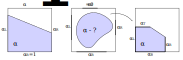
\includegraphics[width=0.8\linewidth]{images/sections/edge_to_area.pdf}
\caption{Восстановление объемной доли в квадрате, по долям на ребрах.\label{fig:edge-to-area}}
\end{figure}
Я покрутил квадраты, итоговая формула получилась следующая:
\begin{multline*}
\alpha= \frac{1}{2} \big[
\min \qty(\alpha_L, \, \alpha_R) \cdot \max \qty(\alpha_B, \, \alpha_T) + 
\max \qty(\alpha_L, \, \alpha_R) \cdot \min \qty(\alpha_B, \, \alpha_T) + \\ +
\max \qty(\alpha_L, \, \alpha_R) \cdot \max \qty(\alpha_B, \, \alpha_T) -
\min \qty(\alpha_L, \, \alpha_R) \cdot \min \qty(\alpha_B, \, \alpha_T)
\big].
\end{multline*}

\subsection{Сечения кубоидов}

1. Сечение единичного куба. Нормаль упорядочена, $|n_x| \le |n_y| \le |n_z|$.




\section{Специальные функции}


Мне надоело каждый раз сочинять одни и те же часто используемые функции. Надо записать. Далее функция Хевисайда $\eta(x)$ доопределена нулем в нуле (!), функция знака $\sgn(x)$. Получается, не связана с $\sgn$.
\medskip

\subsection*{Гладкая функция Хевисайда}

Гладкая функция $f(x)$ определена при значениях $x > 0$. Определим для значений $x \ge 0$ функцию $\hat{f} (x)$ следующим образом: $\hat{f}(0) = 0$ и $\hat{f}(x) \equiv f(x)$ при $x > 0$. Если $\eta(x)$ --- функция Хевисайда, которая в точке $x = 0$ принимает значение 0, тогда функцию $\hat{f}(x)$ можно записать как $\hat{f}(x) = \eta(x) f(x)$\footnote{Фактически, такое соглашение использует Горюнов при работе с обобщенными функциями в области $x \ge 0$. Такое определение $\eta(x)$ позволяет занулять значение функции в нуле, а также брать обобщенную производную и выполнять преобразование Лапласа}. При этом, если $\displaystyle \lim_{x \to 0} f(x) \neq 0$, тогда новая функция $\hat{f}(x)$ имеет скачок в точке $x = 0$. Собственно, если имеется функция $f(x)$, которую необходимо доопределить новым значением в точке $x = 0$, но при этом хочется это сделать <<гладко>>, без скачков, то можно воспользоваться гладкой функцией Хевисайда $\eta_{s} (x)$ (smooth), работаем с ней аналогично $\hat{f}(x) = \eta_s(x) f(x)$.

Что мы будем называть гладкой функцией Хевисайда $\eta_s(x)$? Введем два параметра: $x_0$ --- смещение функции Хевисайда, $w > 0$ --- ширина. Функция $\eta_s(x) = 0$ при $x \le x_0$, функция $\eta(x) = 1$ при $x \ge x_0 + w$. На интервале $x \in [x_0, \, x_0 + w]$ функция изменяется непрерывно. Очевидно, при уменьшении ширины $w \to 0$ гладкая функция Хевисайда стремится к обычной $\eta(x)$. Будем в общем случае писать как $\eta_s(x)$ (smooth), подразумевая, что в функции есть ещё пара параметров $(x_0, \, w)$. Хотя в простейшем случае можно полагать, что $x_0 = 0$ и $w = 1$.
\smallskip

Почему-то первой в голову пришел вариант гладкой функции с синусом. Вероятно, потому что изначально я строил сигмоиды, которые являются нечетными функциями.Обозначим функцию как $\eta_{sin}(x)$:
\begin{equation}
\eta_{sin}(x) = \left\{
\begin{aligned}
&0,                       &&\quad x \le x_0, \\
&\sin \frac{\pi (x - x_0)}{2w},  &&\quad x \in (x_0, \, x_0 + w), \\
&1,                       &&\quad x \ge x_0 + w. 
\end{aligned}
\right.
\end{equation}
\begin{equation*}
\eta_{sin}(x) = \eta(\xi) \cdot \qty(1 + \eta \qty(1 - \xi) \cdot \qty( \sin \frac{\pi \xi}{2} - 1) ), \qquad \xi = \frac{x - x_0}{w}.
\end{equation*}
Равна нулю при $x \le x_0$, выходит на единицу на отрезке $[x_0, \, x_0 + w]$. Функция гладкая в точке $x = x_0 + w$. Второй вариант записи удобен при векторизации в python. Производная в $x_0$:
\begin{equation*}
\lim_{x \to x_0} \eta_{sn}'(x) = \frac{\pi}{2w}.
\end{equation*}
\smallskip

Зачем использовать синус, он ведь долго считается. Можно использовать полином (polinomial). Самое простое --- квадратичный. Обозначим как $\eta_{p2}(x)$:
\begin{equation*}
\eta_{p2}(x) = \left\{
\begin{aligned}
&0,                       &&\quad x \le x_0, \\
&\xi \cdot \qty(2 - \xi), &&\quad x \in (x_0, \, x_0 + w), \\
&1,                       &&\quad x \ge x_0 + w. 
\end{aligned}
\right.
\end{equation*}
Функция $\eta_{p2}(x)$ гладкая в точке $x = x_0 + w$. Потом выяснил, что эту функцию легко обобщить. Можно выбрать не квадратичный полином, а полином степени $n$. Обозначим как функцию $\eta_{pn}(x)$:
\begin{equation}
\eta_{pn}(x) = \left\{
\begin{aligned}
&0,                   &&\quad x \le x_0, \\
&1 - \qty(1 - \xi)^n, &&\quad x \in (x_0, \, x_0 + w), \\
&1,                   &&\quad x \ge x_0 + w. 
\end{aligned}
\right.
\end{equation}
\begin{equation*}
\eta_{pn}(x) = \eta(\xi) \cdot \qty(1 - \eta \qty(1 - \xi) \cdot \qty( 1 - \xi )^{n} ), \qquad \xi = \frac{x - x_0}{w}.
\end{equation*}
Функция $\eta_{pn}(x)$ в точке $x = x_0 + w$ имеет $n - 1$ производную равную нулю, то есть у неё высокая степень гладкости при $x > 0$. Производная в нуле для полиномиальных Хевисайдов зависит от степени $n$:
\begin{equation*}
\lim_{x \to x_0} \eta_{pn}'(x) = \frac{n}{w},
\end{equation*}
это позволяет регулировать наклон в точке $x = x_0$.
\smallskip

Если полиномиальная функция всё равно недостаточно резкая, то можно использовать функцию с бесконечной производной в $x_0$. Простейший способ сконструировать такую функцию это использовать извлечение корня. Обозначим класс функций $\eta_{rn}(x)$ (rational): 
\begin{equation}
\eta_{rn}(x) = \left\{
\begin{aligned}
&0,                       &&\quad x \le x_0, \\
& \frac{1}{n} \sqrt[n]{\xi} \cdot \qty(n + 1 - \xi), &&\quad x \in (x_0, \, x_0 + w), \\
&1,                       &&\quad x \ge x_0 + w. 
\end{aligned}
\right.
\end{equation}
\begin{equation*}
\eta_{rn} (x) = \eta(\xi) \cdot \qty( 1 + \eta(1 - \xi) \cdot \qty( \frac{1}{n} \sqrt[n]{|\xi|} \cdot (n + 1 - \xi) - 1) ), \qquad \xi = \frac{x - x_0}{w}.
\end{equation*} 
Функция $\eta_{rn}(x)$ является гладкой в точке сшивки $x = x_0 + w$. Хотя производная в точке $x = x_0$, показатель корня $n$ влияет на резкость функции. При $n \to \infty$ функция стремится к обычному Хевисайду. На практике, чтобы не тратить много вычислительных ресурсов, следует использовать квадратный или кубический корень.


\subsection*{Гладкая функция знака/сигмоиды}

Меня не устраивают классические функции-сигмоиды, поскольку они выходят на значения -1 и 1 только асимптотически. Мне нужны функции, которые достигают значения 1 по модулю при выходе за установленные рамки.

Что будем называть гладкой функцией знака? Нечетная функция относительно точки $x = x_0$, при значениях $|x - x_0| \ge w$ принимает значение по модулю равное единице. Желательно гладкая. Гладкую функцию знака с таким определением можно ввести через определенные ранее гладкие функции Хевисайда $\eta_s(x)$. Если $x_0 = 0$, тогда определим гладкую функцию знака $\sgn_s(x)$ как $\sgn_s(x) = \sgn(x) \eta_s(|x|)$. Внимание, следует помнить, что между гладкими версиями \textbf{не работает} связь $\sgn(x) + 1 = 2 \eta(x)$.

Сигмоида с синусом:
\begin{equation}
\sgn_{sin}(x) = \left\{
\begin{aligned}
&-1,                       &&\quad x \le x_0 - w, \\
&\sin \frac{\pi (x - x_0)}{2w},  &&\quad | x - x_0 | \le w, \\
&+1,                       &&\quad x \ge x_0 + w. 
\end{aligned}
\right.
\end{equation}
\begin{equation*}
\sgn_{sin}(x) = \eta_{\half} \qty(|\xi| - 1) \cdot \sgn(\xi) + \eta_{\half} \qty(1 - |\xi|) \cdot \sin \frac{\pi \xi}{2}, \qquad \xi = \frac{x - x_0}{w}.
\end{equation*}
\begin{equation*}
\lim_{x \to x_0} \eta_{sn}'(x) = \frac{\pi}{2w}.
\end{equation*}

Полиномиальная сигмоида:
\begin{equation}
\sgn_{pn}(x) = 
\sgn(x - x_0) \cdot
\left\{
\begin{aligned}
&1 - \qty(1 - |\xi|)^n, &&\quad |x - x_0| < w, \\
&1,                     &&\quad |x - x_0| \ge w. 
\end{aligned}
\right.
\end{equation}
\begin{equation*}
\sgn_{pn}(x) = \sgn(\xi) \cdot \qty(1 - \eta \qty(1 - |\xi|) \cdot \qty( 1 - |\xi| )^{n} ), \qquad \xi = \frac{x - x_0}{w}.
\end{equation*}
Функция $\sgn_{pn}(x)$ в точках $x = x_0 \pm w$ имеет $n - 1$ производную равную нулю, то есть у неё высокая степень гладкости в точках $x \neq x_0$. Производная в $x = x_0$ для полиномиальной функции знака зависит от степени $n$, что позволяет регулировать наклон:
\begin{equation*}
\lim_{x \to x_0} \sgn_{pn}'(x) = \frac{n}{w}.
\end{equation*}

Сигмоида с корнем:
\begin{equation}
\sgn_{rn}(x) =
\sgn (x - x_0) \cdot
 \left\{
\begin{aligned}
& \frac{1}{n} \sqrt[n]{|\xi|} \cdot \qty(n + 1 - |\xi|), &&\quad |x - x_0| < w, \\
& 1,                       &&\quad |x - x_0| \ge w. 
\end{aligned}
\right.
\end{equation}
\begin{equation*}
\sgn_{rn} (x) = \sgn(\xi) \cdot \qty( 1 + \eta(1 - |\xi|) \cdot \qty( \frac{1}{n} \sqrt[n]{|\xi|} \cdot (n + 1 - |\xi|) - 1) ), \qquad \xi = \frac{x - x_0}{w}.
\end{equation*} 
Функция $\sgn_{rn}(x)$ является гладкой в точках сшивки $x = x_0 \pm w$. Показатель корня $n$ влияет на резкость функции, при $n \to \infty$ функция стремится к обычной функции знака. На практике, для оптимизации вычислений, следует использовать квадратный или кубический корень.


\chapter{Приложения}



\section{Выкладки}

\subsection{Двучленное уравнение состояния и Stiffened Gas}
\label{app:stiffened}

Стартуем с формулы
\begin{equation}
P(\rho, \, e) = \qty(\gamma - 1) \rho e + c_0^2 \qty(\rho - \rho_0)
\end{equation}
Хотим найти термическое уравнение состояния $P(\rho, \, T)$. Просто так его из $P(\rho, \, e)$ не вывести, требуется хотя бы некоторое допущение. Используем следующее, предполагаем, что $\qty( \dfrac{\partial e}{\partial T} )_{\rho} = c_v = \const$, тогда внутренняя энергия представляется в форме
\begin{equation}
e(\rho, \, T) = c_v T + K( \rho ),
\end{equation}

Попробуем найти каноническое уравнение состояния $e(\rho, \, s)$.
\begin{equation}
\qty( \pdv{e}{s} )_{\rho} = T = \frac{e (\rho, \, s) - K(\rho)}{c_v},
\end{equation}
это что-то вроде ОДУ на $e(\rho, \, s)$, общее решение имеет вид
\begin{equation}
e(\rho, \, s) = A(\rho) \exp \qty( \tfrac{s}{c_v} ) + K(\rho).
\end{equation}

Также известно
\begin{equation}
\qty(\pdv{e}{\rho})_{s} = \frac{P}{\rho^2}.
\end{equation}
Тут уже ОДУ которое должно выполняться тождественно $\forall s$:
\begin{equation}
\rho^2 \qty[ A'(\rho) \exp \qty( \tfrac{s}{c_v} ) + K'(\rho)] = P = \qty(\gamma - 1) \rho \qty[ A(\rho) \exp \qty( \tfrac{s}{c_v} ) + K(\rho)] + c_0^2 \qty(\rho - \rho_0)
\end{equation}
Отсюда можно вычислить $A(\rho)$ и $K(\rho)$, а значит и $e(\rho, \, s)$. Решение содержит только две константы $e_1$ и $e_2$. 
\begin{equation}
A(\rho) = e_1 \exp \qty(\tfrac{s}{c_v}) \qty(\frac{\rho}{\rho_0})^{\gamma - 1},
\qquad
K(\rho) = e_2 \qty(\frac{\rho}{\rho_0})^{\gamma - 1} + \frac{\rho_0 c_0^2}{\gamma \rho} - \frac{c_0^2}{\gamma - 1},
\end{equation}
\begin{equation}
e\qty(\rho, \, s) = \qty[e_1 \exp \qty(\tfrac{s}{c_v}) + e_2] \qty(\frac{\rho}{\rho_0})^{\gamma - 1} + \frac{\rho_0 c_0^2}{\gamma \rho} - \frac{c_0^2}{\gamma - 1}.
\end{equation}

Константа $e_1$ перед экспонентой никак не влияет на формулу для давления. Теперь есть два варианта. 1 это волевым решением положить $e_2 = 0$. Пурурум, получится Stiffened Gas.  
\begin{equation}
e\qty(\rho, \, s) = A \exp \qty(\tfrac{s}{c_v}) \rho^{\gamma - 1} + \frac{P_0}{\rho} + e_0.
\end{equation}

Второй вариант. Выпишем давление:
\begin{multline*}
P = (\gamma - 1) \rho (c_v T + K(\rho)) + c_0^2 (\rho - \rho_0) =
(\gamma - 1) \rho \qty[c_v T + e_2 \qty(\frac{\rho}{\rho_0})^{\gamma - 1} + \frac{\rho_0 c_0^2}{\gamma \rho} - \frac{c_0^2}{\gamma - 1}] + \\ + c_0^2 (\rho - \rho_0) = \qty(\gamma - 1) c_v \rho T + \qty(\gamma - 1) \rho_0 e_2 \qty( \frac{\rho}{\rho_0} )^{\gamma} - \frac{\rho_0 c_0^2}{\gamma} = \\ = \qty(\gamma - 1) c_v \rho T + \frac{\rho_0 c_0^2}{\gamma} \qty[ \frac{\gamma \qty(\gamma - 1) e_2}{c_0^2} \qty( \frac{\rho}{\rho_0} )^{\gamma} - 1].
\end{multline*}
Вторую скобку будем называть <<упругой частью>> давления. Будем выбирать параметр $e_0$ таким образом, чтобы упругая часть давления обращалась в ноль при $\rho = \rho_0$, то есть
\begin{equation}
e_2 = \frac{c_0^2}{\gamma \qty(\gamma - 1)} = - \frac{e_0}{\gamma}.
\end{equation}

Второй вариант канонического уравнения состояния:
\begin{equation}
e\qty(\rho, \, s) = \qty[A \exp \qty(\tfrac{s}{c_v}) - \frac{e_0}{\gamma}] \qty(\frac{\rho}{\rho_0})^{\gamma - 1} + \frac{P_0}{\rho} + e_0.
\end{equation}

Параметр $A$ ни на что не влияет. Пофиг.

\subsection{Ми -- Грюнайзена и Мурнагана}

Будем следовать статье \cite{Heuze12} при выводе общей формы уравнения Ми -- Грюнайзена. В начале 20-го века Ми и Грюнайзен разрабатывали теорию твердых материалов, в которой давление линейная функция энергии. Общее наименование Ми -- Грюнайзена относится к моделям, которые следуют этому допущению. Коэффициент пропорциональности $\Gamma(\rho)$, который связывает энергию и давление называется параметром Грюнайзена.

При исследовании кристаллов они получили, что внутренняя энергия кристаллов складывается из их потенциальной энергии при нулевой температуре (потенциал взаимодействия атомов при нулевой температуре), а также из температурной энергии вибраций, которая растет с температурой
\begin{equation}
e(\rho, \, T) = e_{ref} (\rho) + e_{T} (\rho, \, T),
\end{equation}
Аналогичное разложение используется для давления:
\begin{equation}
P(\rho, \, T) = P_{ref} (\rho) + P_T (\rho, \, T),
\end{equation}
Потенциальная энергия $e_{ref}(\rho)$ также называется холодной энергией или референсным потенциалом, $P_{ref}(\rho)$ --- холодное или референсное давление. Они связаны соотношением
\begin{equation}
P_{ref}(\rho) = \rho^2 e'_{ref} (\rho).
\end{equation}

Референсные кривые при нулевой температуре получаются математически при анализе кристаллических решеток, к примеру, простые формулы приводятся здесь \cite{Lemons99}. Правда математика и теоретическая физика дают очень грубые оценки для констант в уравнениях, так что их потом подбирают в экспериментах. Ну хотя бы вид функций известен.


Температурное давление $P_T(\rho, \, T)$ пропорционально энергии $e_{T} (\rho, \, T)$. Их соотношение не зависит от температуры, а только от вибрационной частоты $\nu$ и плотности $\rho$. Параметр Грюнайзена $\Gamma$ можно ввести как
\begin{equation*}
\Gamma (\rho) = \frac{d \ln \nu}{d \ln \rho}.
\end{equation*}
Исходя из \textit{virial theorem} Грюнайзен получил
\begin{equation}
P(\rho, \, e) - P_{ref} \qty(\rho) = \Gamma (\rho) \rho \, \qty[ e - e_{ref}(\rho) ].
\end{equation}

Что ещё интересного вводится в статье. Ну во первых предположим, что $c_v = \qty(de / dT)_{\rho} = \const$, как часто делаем.
Вот есть формула температуры Дебая
\begin{equation}
T_ref(\rho) = T_0 \cdot \exp \qty[ \int_{\rho_0}^{\rho} \frac{\Gamma(\rho)}{\rho} d \rho ],
\end{equation}
которую будем использовать в качестве референсной кривой.
И известно, свойство, указано в статье \cite{Heuze12}.
\begin{equation}
e - e_{ref}(\rho) = T_{ref}(\rho) \qty[ \sigma (s) - \sigma (s_0)].
\end{equation}
где $\sigma (s)$ -- энтропийная функция.

Откуда берется уравнение состояния из основного раздела? Для референсной кривой выбирается закон Мурнагана.
\begin{equation}
P_{ref} (\rho) = \frac{B}{n} \qty[ \qty( \frac{\rho}{\rho_0} )^{n} - 1].
\end{equation}
Для референсной температуры есть две опции, если предположить $\Gamma = \const$, тогда интегрирование даст
\begin{equation}
T_{ref}(\rho) = T_0 \qty( \frac{\rho}{\rho_0} )^{\Gamma},
\end{equation}
ну то есть как для двучленного уравнения состояния ($\Gamma = \gamma - 1$). Можем также предположить, в \cite{Heuze12} написано, что это стандартное предположение для металлов, что $\Gamma (\rho) \rho = \Gamma \rho_0 = \const$. Тогда после интегрирования получим
\begin{equation}
T_{ref}(\rho) = T_0 \exp \qty[ \Gamma \qty(1 - \frac{\rho_0}{\rho} ) ],
\end{equation}
действительно, такая версия встречается, к примеру, у Уолша и Кристиана \cite{Walsh55}. Во видимому, если выбирать эту версию, то и в основном уравнении следует заменить $\rho$ на $\rho_0$. Последний произвол остался в выборе энтропийной функции. Ну тут выбираем как обычно, откуда это следует, я пока не разобрался. Кажется из того что $c_v = \const$
\begin{equation}
\sigma(s) = \exp \qty( \tfrac{s - s_0}{c_v} ).
\end{equation}
Тогда каноническое уравнение состояния:
\begin{equation}
e = e_{ref}(\rho) + c_v T_{ref}(\rho) \qty( \exp \qty( \tfrac{s - s_0}{c_v} ) - 1).
\end{equation}







\bibliography{library.bib}


\end{document} 
